\documentclass[12pt]{article}
\usepackage{amsmath}
\usepackage{relsize}
\usepackage{mdframed}
\usepackage{texmaths-tikz}
\usepackage{tikz}
\usepackage{geometry}
\usepackage{tabularray}

\usetikzlibrary{3d,backgrounds,perspective}

\newgeometry{
    % includehead,
    lmargin=10pt,
    textwidth=595pt,
    % textwidth=\page@width,
    top=1cm,
    % headsep=\page@vtop@sep,
    % headheight=\page@head@height,
    % textheight=\page@textheight,
    % footskip=2\page@vtop@sep
}

\def\guillemets#1{\guillemotleft\ #1\ \guillemotright}
\long\def\next{\medskip\par\noindent}
\def\PP#1{\displaystyle\mathcal{P}_\text{\ #1}}
\def\AA#1{\displaystyle\mathcal{A}_\text{\ #1}}
\def\VV#1{\displaystyle\mathcal{V}_\text{\ #1}}
\def\palette{Rainbow1}

\global\mdfdefinestyle{longueur}{%
    linecolor=\palette-rouge,linewidth=3pt,%
    leftmargin=1cm,rightmargin=1cm,
    frametitlerule=true,frametitlerulecolor=\palette-rouge,
    frametitlebackgroundcolor=\palette-jaune,
    frametitlerulewidth=2pt
}
\global\mdfdefinestyle{surface}{%
    linecolor=\palette-bleu,linewidth=3pt,%
    leftmargin=1cm,rightmargin=1cm,
    frametitlerule=true,frametitlerulecolor=\palette-bleu,
    frametitlebackgroundcolor=\palette-jaune,
    frametitlerulewidth=2pt
}
\global\mdfdefinestyle{volume}{%
    linecolor=\palette-vert,linewidth=3pt,%
    leftmargin=1cm,rightmargin=1cm,
    frametitlerule=true,frametitlerulecolor=\palette-vert,
    frametitlebackgroundcolor=\palette-jaune,
    frametitlerulewidth=2pt
}
\tikzset{every picture/.style={line width=1.5pt}}
\begin{document}\thispagestyle{empty}
\begin{mdframed}[style=longueur,frametitle={$\mathcal{P}$érimètre
    (\normalfont la longueur du contour)}]
    $\PP{polygone}=\text{somme des côtés}$\next
    $\PP{cercle}=\text{diamètre}\times\pi$
\end{mdframed}
\begin{mdframed}[style=longueur,frametitle={Longueurs}]
    \begin{tblr}{colspec=*{2}{Q[c,m,wd=230pt]}}
        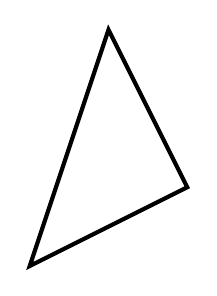
\begin{tikzpicture}
            \draw(0,0)--(2,1)--(1,3)--cycle;
        \end{tikzpicture}&
        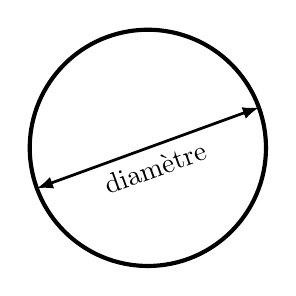
\begin{tikzpicture}\def\rayon{1.5}
            \draw(0,0)circle(\rayon);
            \coordinate(A)at(200:\rayon);
            \coordinate(B)at(20:\rayon);
            \draw[latex-latex,line width=1pt](A)--(B);
            \path(B)--(A)node[midway,sloped,below]{diamètre};
        \end{tikzpicture}\\
        Polygone&Cercle\\
    \end{tblr}
\end{mdframed}
\begin{mdframed}[style=surface,frametitle={$\mathcal{A}$ire (\normalfont
    surface à l'intérieur)}]
    $\AA{parallélogramme}=\text{base}\times\text{hauteur}$\next
    $\AA{rectangle}=\text{longueur}\times\text{largeur}$\next
    $\AA{triangle}=\text{base}\times\text{hauteur}\div2$\next
    $\AA{disque}=\pi\times\text{rayon}\times\text{rayon}$
\end{mdframed}

\begin{mdframed}[style=surface,frametitle={Surfaces}]
    \def\delay{0.25}
    \def\pardec{0.75}
    \def\lenght{3}
    \def\height{2.5}
    \def\rayon{2}
    \begin{tblr}{colspec=*{4}{Q[c,m,wd=115pt]}}
        \begin{tikzpicture}
            \coordinate(A)at(0,0);
            \coordinate(B)at(\lenght,0);
            \path(A)+(0,-\delay)coordinate(A');
            \path(B)+(0,-\delay)coordinate(B');
            \coordinate(D)at(\pardec,\height);
            \coordinate(D')at(\pardec,0);
            \coordinate(C)at(\lenght+\pardec,\height);
            \filldraw[\palette-jaune,draw=black](A)--(B)--(C)--(D)--cycle;
            \draw[latex-latex,line width=1pt](A')--(B');
            \path(A')--(B')node[midway,sloped,below]{\small base};
            \draw[latex-latex,line width=1pt](D)--(D');
            \path(D')--(D)node[midway,sloped,below]{\small hauteur};
        \end{tikzpicture}&
        \begin{tikzpicture}
            \coordinate(A)at(0,0);
            \coordinate(B)at(\lenght,0);
            \path(A)+(0,-\delay)coordinate(A');
            \path(B)+(0,-\delay)coordinate(B');
            \coordinate(D)at(\pardec,\height);
            \coordinate(D')at(\pardec,0);
            \coordinate(C)at(\lenght+\pardec,\height);
            \filldraw[\palette-jaune,draw=black](A)--(B)--(D)--cycle;
            \draw[latex-latex,line width=1pt](A')--(B');
            \path(A')--(B')node[midway,sloped,below]{\small base};
            \draw[latex-latex,line width=1pt](D)--(D');
            \path(D')--(D)node[midway,sloped,below]{\small hauteur};
        \end{tikzpicture}&
        \begin{tikzpicture}
            \coordinate(A)at(0,0);
            \coordinate(B)at(\lenght,0);
            \path(A)+(0,-\delay)coordinate(A');
            \coordinate(D)at(0,\height);
            \path(B)+(0,-\delay)coordinate(B');
            \path(B)+(\delay,0)coordinate(B'');
            \coordinate(C)at(\lenght,\height);
            \path(C)+(\delay,0)coordinate(C');
            \filldraw[\palette-jaune,draw=black](A)--(B)--(C)--(D)--cycle;
            \draw[latex-latex,line width=1pt](A')--(B');
            \path(A')--(B')node[midway,sloped,below]{\small longueur};
            \draw[latex-latex,line width=1pt](B'')--(C');
            \path(B'')--(C')node[midway,sloped,below]{\small largeur};
        \end{tikzpicture}&
        \begin{tikzpicture}[scale=0.75,baseline=(B.base)]
            \filldraw[fill=\palette-jaune,draw=black](0,0)circle(\rayon);
            \coordinate(A)at(20:\rayon);
            \coordinate(B)at(0,-1.4*\rayon);
            \draw[latex-latex,line width=1pt](0,0)--(A);
            \path(0,0)--(A)node[midway,sloped,below]{\small rayon};
        \end{tikzpicture}
            \\
            Parallélogramme&Triangle&Rectangle&Disque\\
        \end{tblr}
    \end{mdframed}
% \newpage
% \begin{mdframed}[style=volume,frametitle={$\mathcal{V}$olume \normalfont
%     (espace à l'intérieur)}]
%     $\VV{prisme ou cylindre}=\AA{base}\times\text{hauteur}$\next
%     $\VV{pyramide ou cône}=\AA{base}\times\text{hauteur}\div3$\next
%     $\VV{boule}=\dfrac43\pi\times\text{rayon}\times\text{rayon}\times\text{rayon}$
% \end{mdframed}


\end{document}

